\documentclass[10pt,twocolumn,letterpaper]{article}
\usepackage[margin=1.8cm, columnsep=0.6cm]{geometry}

% 引入全局宏包与数学符号定义
% =========================================================================
% macros.tex - 全局学术宏包、专用数学符号与图表高亮命令
% =========================================================================

% 基础数学与字体支持
\usepackage{amsmath,amssymb,amsfonts}
\usepackage{bm}                       % 粗体数学符号
\usepackage{graphicx}
% Keep referenced floats within their discussion before the conclusion.
\usepackage{placeins}
\usepackage{booktabs}                 % 标准三线表 (\toprule, \midrule, \bottomrule)
\usepackage{multirow}
\usepackage{makecell}
\usepackage{array}
\usepackage{xcolor}
\usepackage{colortbl}

% 顶刊紧凑版面微调
\let\Bbbk\relax                       % 避免符号冲突
\usepackage{newtxtext,newtxmath}
\usepackage[font=small,labelfont=bf,labelsep=period]{caption}
\usepackage[font=footnotesize]{subcaption}

% 交叉引用与超链接
\usepackage[pagebackref,breaklinks,colorlinks,citecolor=blue,linkcolor=red]{hyperref}
\usepackage[capitalize]{cleveref}
\usepackage{pgfplots}

% 常用学术缩写
\newcommand{\etal}{\textit{et al.}}
\newcommand{\ie}{\textit{i.e.}}
\newcommand{\eg}{\textit{e.g.}}
\newcommand{\wrt}{\textit{w.r.t.}}

% 表格指标高亮
\newcommand{\best}[1]{\textbf{\textcolor{red}{#1}}}
\newcommand{\second}[1]{\underline{\textcolor{blue}{#1}}}

% 图像与空间定义
\newcommand{\R}{\mathbb{R}}
\newcommand{\Iir}{\mathbf{I}_{\text{ir}}}       % 红外源图像
\newcommand{\Ivis}{\mathbf{I}_{\text{vis}}}     % 可见光源图像
\newcommand{\Ifuse}{\mathbf{I}_{\text{f}}}      % 最终融合图像
\newcommand{\Irec}{\hat{\mathbf{I}}}            % Phase I 自编码重构图像

% 多阶段特征张量表达
\newcommand{\Fsh}{\bm{\Phi}^{\text{S}}}         % 浅层共享特征 (Stage 1)
\newcommand{\Fbase}{\bm{\Phi}^{\text{B}}}       % 低频基底特征 (Stage 2A)
\newcommand{\Fdet}{\bm{\Phi}^{\text{D}}}        % 高频细节特征 (Stage 2B)

% 网络组件算子
\newcommand{\Eshared}{\mathcal{E}_{\text{stem}}}
\newcommand{\Ebase}{\mathcal{E}_{\text{B}}}
\newcommand{\Edetail}{\mathcal{E}_{\text{D}}}
\newcommand{\Drec}{\mathcal{D}}
\newcommand{\FfuseB}{\mathcal{F}_{\text{B}}}
\newcommand{\FfuseD}{\mathcal{F}_{\text{D}}}

% 损失函数符号体系
\newcommand{\Ltotal}{\mathcal{L}_{\text{total}}}
\newcommand{\Ldecomp}{\mathcal{L}_{\text{decomp}}^{\text{ortho}}}
\newcommand{\Lintra}{\mathcal{L}_{\text{intra}}}
\newcommand{\Lfusion}{\mathcal{L}_{\text{fusion}}}
\newcommand{\Lin}{\mathcal{L}_{\text{in}}}
\newcommand{\Lgrad}{\mathcal{L}_{\text{grad}}}
\newcommand{\Lstruct}{\mathcal{L}_{\text{struct}}}
\newcommand{\Lsd}{\mathcal{L}_{\text{sd}}}
\newcommand{\CC}{\operatorname{CC}}             % 皮尔逊相关系数

\pgfplotsset{compat=1.18}


% ==================== 论文标题与作者信息 ====================
\title{\vspace{-1.0cm}\Large\bfseries SCMFuse: Efficient Space--Channel Mamba Fusion for Infrared and Visible Images}

\author{
    \normalsize Wenbin Li$^{1}$ \\[0.3em]
    \small $^{1}$Jiangnan University \\
    {\tt\footnotesize 6243111035@Jiangnan.edu.cn}
}
\date{\vspace{-1.5em}}

\begin{document}
\maketitle

% ==================== 0. 摘要与关键词 ====================
\begin{abstract}
\noindent\small
Infrared and visible image fusion must preserve thermal targets and visible structures while limiting computational cost. We propose SCMFuse, an efficient dual-branch framework that combines local feature extraction, space--channel modeling, and contrast--structure supervision. Multi-scale gated convolutions reduce the cost of shallow encoding and reconstruction. A space--channel MambaVision block combines four-directional scanning in a pooled path with full-resolution residual features and transposed channel attention. Difference- and magnitude-guided gates adapt the aggregation of base and detail representations. The training objective adds intra-modal decorrelation, local structural correlation, and global--local contrast regularization while retaining maximum-intensity and Sobel-gradient targets. Experiments on MSRS, TNO, and RoadScene show improved structural correlation relative to CDDFuse across all three datasets, with higher visual information fidelity and edge transfer quality on TNO and RoadScene. The model uses $0.473$ M parameters and $87.837$ G FLOPs under the reported profile, reductions of $60.2\%$ and $62.7\%$, respectively. The full configuration provides $1.56\times$ training acceleration and $2.76\times$ mean inference speedup. These results demonstrate a practical balance between computational efficiency and the preservation of complementary image information.


\vspace{0.4em}
\noindent\textbf{Keywords:} Infrared and visible image fusion, state space model, MambaVision, feature decorrelation, gated fusion, contrast preservation.
\end{abstract}
\vspace{0.5em}

% ==================== 1~5. 正文各章节模块化引入 ====================
\section{Introduction}\label{sec:intro}
Infrared and visible sensors capture different aspects of a scene. Visible images describe reflected-light appearance and texture, but their quality depends on illumination. Infrared images reveal thermal patterns that remain useful in low-light environments, although they often contain less appearance detail. Infrared and visible image fusion (IVIF) combines these complementary observations into a single image, with applications in nighttime perception and scene monitoring~\cite{ma2019survey,tang2022seafusion}. An effective method must preserve thermal targets and visible structures while keeping computation manageable.

Deep learning has advanced this task through convolutional feature extraction, auto-encoding, adversarial learning, and attention-based modeling~\cite{li2019densefuse,xu2022u2fusion,ma2019fusiongan,ma2022swinfusion}. Feature-decomposition methods provide a useful way to organize the information to be fused. DIDFuse~\cite{zhao2020didfuse} separates background and detail representations, and CDDFuse~\cite{zhao2023cddfuse} uses a correlation-driven dual-branch design to encourage shared base features and complementary details. Its reconstruction-then-fusion training provides a strong foundation, but leaves room to improve how computation is allocated and how fusion quality is supervised.

We focus on three connected issues. The first is the cost of full-resolution processing. CDDFuse uses Restormer-style blocks for shallow encoding and reconstruction. Their transposed attention efficiently models channel relationships without constructing a quadratic spatial attention matrix~\cite{zamir2022restormer}; nevertheless, repeated projections and feed-forward transformations still contribute substantial computation. Since local boundaries and textures are central to these stages, lightweight gated convolutions offer a way to reduce cost while retaining richer context modeling in the base branch.

The second issue is combining spatial context with channel relationships. Transposed attention derives channel interactions from features aggregated over the image. Selective state-space models offer a complementary route by propagating information through spatial sequences~\cite{gu2023mamba,liu2024vmamba}. Recent fusion methods have explored Mamba for feature enhancement and cross-modal interaction~\cite{xie2024fusionmamba,li2024mambadfuse}. For dense fusion, however, context aggregation should coexist with a direct path for full-resolution features. This motivates a pooled scanning path anchored to a full-resolution residual stream, followed by channel attention. Difference-guided fusion (DGF) and magnitude-guided fusion (MGF) then use cross-modal differences and feature magnitudes to adjust base and detail aggregation, respectively.

The third issue is the balance between intensity, edges, structure, and contrast. Maximum-intensity and gradient targets give useful supervision, but do not explicitly regularize normalized local correlation or global and local intensity variation. The lack of a unique fused ground truth makes this balance consequential: different objectives emphasize different image properties~\cite{zhao2025freefusion}. We retain the original intensity and gradient targets and add complementary structure and contrast terms. An intra-modal decorrelation penalty also discourages redundant patterns between the learned base and detail representations.

We therefore propose SCMFuse, an efficient space--channel Mamba fusion framework. It combines multi-scale local processing, hybrid spatial--channel modeling, adaptive feature aggregation, and targeted supervision within the CDDFuse decomposition paradigm. The main contributions are:
\begin{itemize}
 \item \textbf{Efficient local processing.} A shallow gated convolution block (SGC Block) and a hybrid decoder reduce the computation used for full-resolution feature extraction and reconstruction.
 \item \textbf{Spatial--channel modeling with adaptive fusion.} A space--channel MambaVision block (SCM Block) integrates four-directional spatial scanning, full-resolution residual features, and channel attention. Difference- and magnitude-guided fusion adapt the aggregation of base and detail features.
 \item \textbf{Complementary training constraints.} Intra-modal decorrelation and contrast--structure regularization complement the baseline decomposition and fusion objectives. Experiments on three datasets demonstrate improvements in structural correlation and cross-dataset edge fidelity alongside substantial model compression and acceleration.
\end{itemize}
The full model uses $0.473$ M parameters and $87.837$ G FLOPs, reducing the corresponding CDDFuse profile by $60.2\%$ and $62.7\%$. Its $2.76\times$ mean inference speedup and improved TNO/RoadScene fidelity illustrate the benefit of allocating computation according to the roles of local extraction, global context, and feature aggregation.

\section{Related Work}\label{sec:related}

\subsection{Infrared and Visible Image Fusion}
Early deep fusion methods used auto-encoders and convolutional networks to learn source representations. DenseFuse~\cite{li2019densefuse} combines dense feature extraction with feature-level fusion, while SDNet~\cite{zhang2021sdnet} and U2Fusion~\cite{xu2022u2fusion} investigate learned representations and unsupervised objectives for multiple fusion tasks. FusionGAN~\cite{ma2019fusiongan} and TarDAL~\cite{liu2022tardal} introduce adversarial or target-aware supervision. PIAFusion~\cite{tang2022piafusion} adapts fusion to illumination, and SeAFusion~\cite{tang2022seafusion} connects image fusion with semantic perception. Their objectives reflect different priorities, including source reconstruction, target visibility, and semantic consistency.

Feature decomposition makes the organization of complementary information explicit. DIDFuse~\cite{zhao2020didfuse} learns background and detail features, and CDDFuse~\cite{zhao2023cddfuse} couples a Transformer-based base branch with an invertible neural network (INN) detail branch using cross-modal correlation constraints. More recently, FreeFusion~\cite{zhao2025freefusion} explores cross-reconstruction learning to reduce dependence on handcrafted fusion losses. Our work retains CDDFuse's two-stage decomposition framework and studies a compact architecture with additional feature decorrelation and image-domain regularization.

\subsection{Attention and Efficient Local Processing}
Attention provides content-dependent relationships for restoration and fusion. SwinFusion~\cite{ma2022swinfusion} combines intra-domain and inter-domain interactions through shifted-window attention. Restormer~\cite{zamir2022restormer} uses multi-DConv head transposed attention (MDTA) to estimate channel relationships from spatially aggregated features, avoiding the large pairwise spatial attention maps of conventional self-attention. FC-Former~\cite{wu2025fcformer} further investigates connections across attention modes for multi-source fusion. These studies motivate treating spatial interactions and channel relationships as complementary modeling choices.

Convolutional designs such as NAFNet~\cite{chen2022simple} show the value of efficient local operators in image restoration. Following this direction, our SGC Block combines multi-scale depthwise convolutions with gating and channel reweighting. We use it for shallow extraction and reconstruction, while reserving directional state-space processing and channel attention for the base branch. The focus is the allocation of operations across the fusion pipeline.

\subsection{State-Space Models for Visual Fusion}
Mamba~\cite{gu2023mamba} enables input-dependent sequence modeling with linear scaling in sequence length for fixed model dimensions. VMamba~\cite{liu2024vmamba} adapts scanning to visual data, and EfficientVMamba~\cite{pei2025efficientvmamba} explores efficient scan patterns. MambaIR~\cite{guo2024mambair} combines state-space processing with visual feature refinement, while MambaVision~\cite{hatamizadeh2025mambavision} studies a hybrid Mamba--Transformer backbone. Together, these works suggest combining spatial state propagation with local and channel-based processing.

For fusion, FusionMamba~\cite{xie2024fusionmamba} uses dynamic feature enhancement and cross-modal Mamba interaction. MambaDFuse~\cite{li2024mambadfuse} combines feature extraction with shallow and deep fusion. SCMFuse instead adapts hybrid spatial--channel modeling to a compact dual-branch decomposition network. Its scan path operates at reduced resolution, while an anchor and local path retain full-resolution features. DGF and MGF then use differences and magnitudes to guide feature aggregation. Our focus is how these operations can be integrated within a compact decomposition framework and evaluated through fusion quality and computational cost.

\section{Methodology}\label{sec:method}


\begin{figure*}[!t]
 \centering
 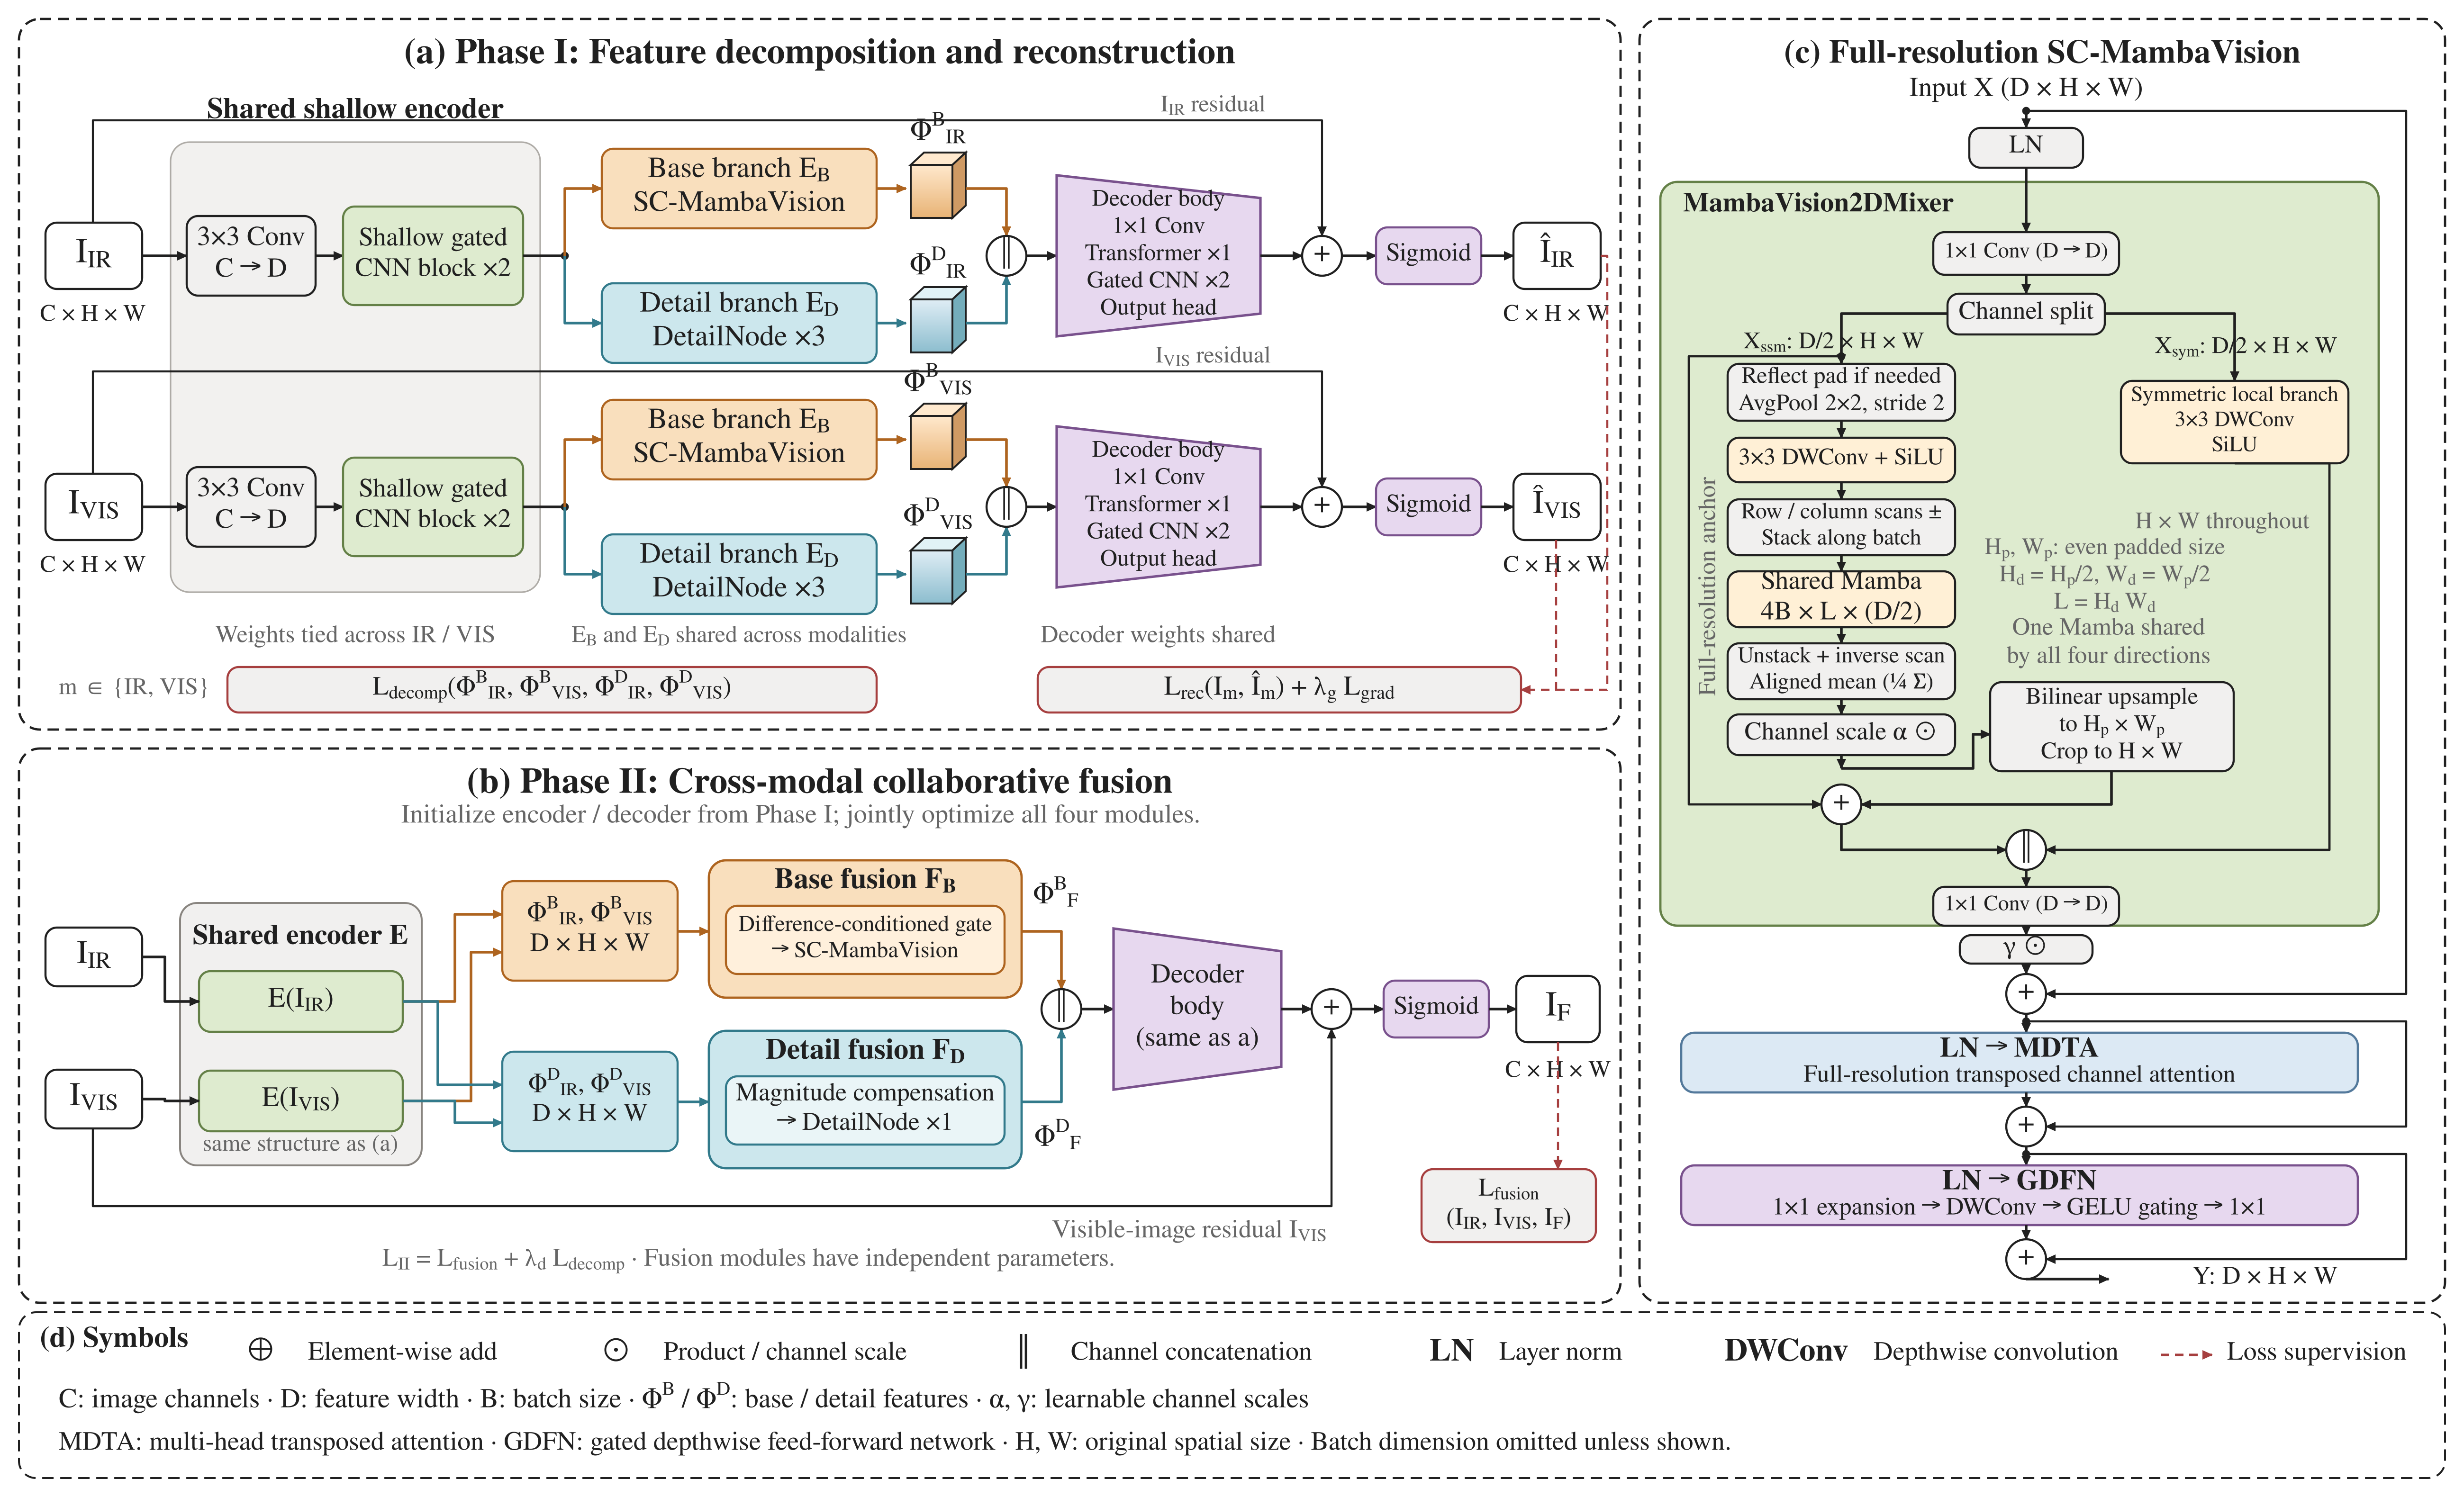
\includegraphics[width=\textwidth]{figs/pipeline.png}
 \caption{Architecture of SCMFuse. (a) Phase I learns base and detail representations by reconstructing each source image with shared encoder and decoder weights. (b) Phase II initializes these components from Phase I and trains cross-modal fusion jointly. (c) The SCM Block combines pooled four-directional scanning, full-resolution residual features, and transposed channel attention. (d) Symbol definitions. The shallow gated CNN block, SC-MambaVision, and MambaVision2DMixer are referred to as SGC Block, SCM Block, and 2D-MV Mixer in the text; base and detail fusion are denoted by DGF and MGF.}
 \label{fig:pipeline}
\end{figure*}

\subsection{Overview}\label{subsec:overall_arch}
Given a registered infrared image $\Iir\in\R^{B\times1\times H\times W}$ and the luminance of a visible image $\Ivis$ with the same dimensions, SCMFuse predicts a fused luminance image $\Ifuse$. Here $B$ is the batch size, $H\times W$ is the spatial resolution, and $D=64$ denotes the feature width. As shown in \cref{fig:pipeline}, the network follows the dual-branch decomposition framework of CDDFuse~\cite{zhao2023cddfuse}:
\begin{equation}
\begin{aligned}
 \Fsh_m&=\Eshared(\mathbf I_m),\\
 (\Fbase_m,\Fdet_m)&=(\Ebase(\Fsh_m),\Edetail(\Fsh_m)),\\
 \Fbase_{\mathrm f}&=\FfuseB(\Fbase_{\mathrm{ir}},\Fbase_{\mathrm{vis}}),\\
 \Fdet_{\mathrm f}&=\FfuseD(\Fdet_{\mathrm{ir}},\Fdet_{\mathrm{vis}}),
\end{aligned}\label{eq:framework}
\end{equation}
where $m\in\{\mathrm{ir},\mathrm{vis}\}$. The encoder and decomposition branches share weights across modalities. Base and detail features are learned representations encouraged to capture shared structure and complementary details; they are not fixed frequency-filter outputs.

We use a \emph{shallow gated convolution block} (\textbf{SGC Block}) for efficient local processing. The base branch uses a \emph{space--channel MambaVision block} (\textbf{SCM Block}), while the detail branch retains the INN-based design of CDDFuse. The fusion layers use \emph{difference-guided fusion} (\textbf{DGF}) for base features and \emph{magnitude-guided fusion} (\textbf{MGF}) for detail features. A hybrid decoder reconstructs the output from the two fused streams. Architectural specifications are summarized in \cref{tab:tensor_dimensions}.

Training has two phases. Phase I learns feature decomposition through source-image reconstruction. Phase II initializes the encoder and decoder from Phase I and learns cross-modal fusion with the proposed supervision. The training phases are distinct from the model configurations evaluated in \cref{subsec:ablation_study}.


\begin{table}[!t]
\centering
\caption{Network specification. All feature maps retain $H\times W$ except inside the scan path. $D=64$; base and detail inputs to the decoder are concatenated.}
\label{tab:tensor_dimensions}
\small
\setlength{\tabcolsep}{3pt}
\begin{tabular}{@{}llc@{}}
\toprule
Component & Main operations & Channels\\
\midrule
Shared encoder & $3\times3$ conv., $2\times$ SGC & $1\to D$\\
Base branch & SCM Block & $D\to D$\\
Detail branch & $3\times$ detail node & $D\to D$\\
Base fusion & DGF, SCM refinement & $2D\to D$\\
Detail fusion & MGF, $1\times$ detail node & $2D\to D$\\
Hybrid decoder & MDTA block, $2\times$ SGC & $2D\to1$\\
\bottomrule
\end{tabular}
\end{table}


\subsection{Efficient Local Processing}
\label{subsec:shallow_encoder}
Full-resolution feature processing is important for dense reconstruction but can account for substantial computation. We use SGC Blocks to capture local patterns with multi-scale depthwise convolutions and retain one transposed-attention block in the decoder to mix base and detail channels. This allocation reduces the repeated attention-based processing used in the baseline encoder and decoder.

\textbf{SGC Block.}
Given $\mathbf X\in\R^{B\times D\times H\times W}$, a point-wise projection expands the normalized features to $2D$ channels and splits them into two streams:
\begin{equation}
 [\mathbf X_a,\mathbf X_b]=\operatorname{Split}
 \big(P_{\mathrm{in}}(\operatorname{LN}(\mathbf X))\big).
\end{equation}
Here $P_{\mathrm{in}}$ is a $1\times1$ convolution and LN denotes layer normalization across channels at each spatial position. The two streams use different kernel sizes:
\begin{equation}
 \mathbf G=\operatorname{SiLU}(\operatorname{DW}_{3}(\mathbf X_a))
              \odot\operatorname{DW}_{5}(\mathbf X_b),
\end{equation}
where $\operatorname{DW}_k$ is a $k\times k$ depthwise convolution and $\odot$ denotes element-wise multiplication. The multiplicative gate combines local responses from the two receptive fields. Channel reweighting and residual refinement then give
\begin{equation}
\begin{aligned}
 \mathbf a&=\sigma\big(P_{\mathrm{ca}}(\operatorname{GAP}(\mathbf G))\big),\\
 \mathbf X'&=\mathbf X+P_{\mathrm{out}}(\mathbf G\odot\mathbf a),\\
 \operatorname{SGC}(\mathbf X)&=\mathbf X'+\operatorname{GDFN}(\operatorname{LN}(\mathbf X')),
\end{aligned}
\end{equation}
where GAP is global average pooling, $P_{\mathrm{ca}}$ and $P_{\mathrm{out}}$ are point-wise convolutions, and $\sigma$ is the sigmoid function. GDFN is the gated depthwise feed-forward network inherited from Restormer~\cite{zamir2022restormer}. A $3\times3$ input convolution followed by two SGC Blocks forms $\Eshared$.

\textbf{Hybrid decoder.}
The decoder concatenates the fused base and detail features and projects them to $D$ channels. It applies one Restormer-style block with multi-DConv head transposed attention (MDTA), followed by two SGC Blocks. The output head contains two $3\times3$ convolutions separated by a LeakyReLU activation. Denoting this reconstruction path by $\mathcal R$, the fused image is
\begin{equation}
 \Ifuse=\sigma\big(\mathcal R([\Fbase_{\mathrm f},\Fdet_{\mathrm f}])+\Ivis\big).
\end{equation}
In Phase I, the same decoder reconstructs each modality using its own source-image residual. The visible residual is used for fusion in Phase II.

\subsection{Space--Channel Base Modeling}\label{subsec:mamba_branch}
MDTA estimates channel relationships from spatially aggregated features, whereas state-space scanning propagates information along spatial sequences. The SCM Block combines these complementary operations. Its residual stream remains at $H\times W$, while pooling is confined to the scanning path.

\textbf{SCM Block.}
For an input feature $\mathbf X$, the block performs
\begin{equation}
\begin{aligned}
 \mathbf X_1&=\mathbf X+\boldsymbol\gamma\odot\mathcal M(\operatorname{LN}(\mathbf X)),\\
 \mathbf X_2&=\mathbf X_1+\operatorname{MDTA}(\operatorname{LN}(\mathbf X_1)),\\
 \operatorname{SCM}(\mathbf X)&=\mathbf X_2+\operatorname{GDFN}(\operatorname{LN}(\mathbf X_2)),
\end{aligned}\label{eq:scm}
\end{equation}
where $\mathcal M$ denotes the two-dimensional MambaVision mixer (\textbf{2D-MV Mixer}) and $\boldsymbol\gamma\in\R^{1\times D\times1\times1}$ is initialized to $0.2$. The base extractor $\Ebase$ uses this block.

\textbf{2D-MV Mixer.}
A point-wise projection splits its input into $\mathbf X_s$ and $\mathbf X_l$, each with $D/2$ channels. The local path processes features at the original resolution:
\begin{equation}
 \mathbf Y_l=\operatorname{SiLU}(\operatorname{DW}_{3}(\mathbf X_l)).
\end{equation}
The spatial path retains $\mathbf X_s$ as an anchor and computes context on a pooled feature map:
\begin{equation}
 \mathbf U=\operatorname{SiLU}\!\left(\operatorname{DW}_{3}
 \big(\operatorname{AvgPool}_{2}(\mathcal P(\mathbf X_s))\big)\right),
\end{equation}
where $\mathcal P$ uses reflection padding to make odd spatial dimensions even. The pooled size is $H_d\times W_d$, with $H_d=\lceil H/2\rceil$ and $W_d=\lceil W/2\rceil$.

The four scan orders are row-major forward/reverse and column-major forward/reverse. Let $\mathcal T_k$ flatten the pooled map in order $k$, and let $\mathcal T_k^{-1}$ restore its spatial layout. All four sequences have length $L=H_dW_d$ and share one Mamba operator~\cite{gu2023mamba}:
\begin{equation}
 \mathbf Y_k=\mathcal T_k^{-1}
 \big(\operatorname{Mamba}(\mathcal T_k(\mathbf U))\big),
 \quad k=1,\ldots,4.
\end{equation}
The directions are stacked along the batch dimension for processing, then spatially aligned and averaged. With a learned channel scale $\mathbf s$, the output is
\begin{equation}
\begin{aligned}
 \mathbf Y_s&=\mathbf X_s+\mathcal U_{H,W}
       \left(\mathbf s\odot\frac14\sum_{k=1}^{4}\mathbf Y_k\right),\\
 \mathcal M(\mathbf X)&=P_{\mathrm m}([\mathbf Y_s,\mathbf Y_l]),
\end{aligned}\label{eq:mixer}
\end{equation}
where $\mathcal U_{H,W}$ uses bilinear interpolation to the padded size and crops to $H\times W$. The learned scale replaces an additional channel normalization at the scan output, leaving relative spatial amplitudes available to subsequent processing.

For even dimensions, each directional sequence has $HW/4$ tokens. The anchor and local path preserve a direct full-resolution route around this pooled computation. MDTA then learns channel interactions from all spatial positions. This combination follows the hybrid modeling motivation of MambaVision~\cite{hatamizadeh2025mambavision}, with directional scanning adapted to image features~\cite{liu2024vmamba}.

\subsection{Difference- and Magnitude-Guided Fusion}
\label{subsec:gated_fusion}
The fusion layers start from additive anchors and learn corrections from cross-modal feature differences. Their refinement modules follow the base and detail branch architectures but use independent weights.

\textbf{DGF for base features.}
Let $\mathbf B_i=\Fbase_{\mathrm{ir}}$ and $\mathbf B_v=\Fbase_{\mathrm{vis}}$. The gate uses both features and their absolute difference:
\begin{equation}
\begin{aligned}
 \mathbf Z_B&=[\mathbf B_i,\mathbf B_v,|\mathbf B_i-\mathbf B_v|],\\
 [\mathbf U_i,\mathbf U_v]&=\mathcal G_B(\mathbf Z_B),\\
 \mathbf W_m&=\mathbf1+\boldsymbol\gamma_B\odot\tanh(\mathbf U_m),
 \quad m\in\{i,v\},\\
 \Fbase_{\mathrm f}&=\operatorname{SCM}_{\mathrm f}
            (\mathbf W_i\odot\mathbf B_i+\mathbf W_v\odot\mathbf B_v).
\end{aligned}
\end{equation}
The gate $\mathcal G_B$ comprises point-wise, depthwise $3\times3$, GELU, and point-wise operations. The shared channel scale $\boldsymbol\gamma_B$ is initialized to $0.1$, so the initial aggregation stays close to addition while allowing modality-dependent corrections.

\textbf{MGF for detail features.}
For $\mathbf D_i=\Fdet_{\mathrm{ir}}$ and $\mathbf D_v=\Fdet_{\mathrm{vis}}$, the magnitude sum provides a cue that remains large when features have opposing signs:
\begin{equation}
\begin{aligned}
 \mathbf Z_D&=[\mathbf D_i,\mathbf D_v,|\mathbf D_i|+|\mathbf D_v|],\\
 \mathbf D_0&=\mathbf D_i+\mathbf D_v+
                  \boldsymbol\gamma_D\odot\mathcal G_D(\mathbf Z_D),\\
 \Fdet_{\mathrm f}&=\operatorname{INN}_1(\mathbf D_0).
\end{aligned}
\end{equation}
Here $\mathcal G_D$ uses the same convolutional pattern as $\mathcal G_B$ with SiLU in place of GELU, and $\boldsymbol\gamma_D$ is initialized to $0.1$. The final refinement uses one detail node, whereas the encoder detail branch contains three nodes. The magnitude cue helps the gate recognize signed-feature disagreement without imposing a fixed sign correction.

\subsection{Training Objectives}\label{subsec:loss_functions}
% Loss primitives: audit/loss_exp4.py. Phase-wise assembly: editorial_review/source_snapshot/models/cddfuse_model.py; configuration: configs/mode/train.yaml in the same snapshot.
The supervision complements reconstruction and cross-modal decomposition with intra-modal decorrelation and image-domain contrast--structure regularization. The new loss components have no trainable inference layers.

\textbf{Feature decorrelation.}
Following CDDFuse, the cross-modal term favors correlated base features and decorrelated detail features. We add an intra-modal penalty:
\begin{equation}
 \Ldecomp=\frac{\CC(\Fdet_{\mathrm{vis}},\Fdet_{\mathrm{ir}})^2}
 {1.01+\CC(\Fbase_{\mathrm{vis}},\Fbase_{\mathrm{ir}})}
 +\lambda_{\mathrm{ortho}}\Lintra.
\end{equation}
The operator $\CC$ is the baseline feature-correlation routine. For each modality, image, and channel, base and detail maps are centered over their spatial positions. With the centered vectors denoted by $\tilde{\mathbf b}_{m,b,c}$ and $\tilde{\mathbf d}_{m,b,c}$, we use
\begin{equation}
 \Lintra=\frac{1}{2BD}\sum_{m,b,c}
 \frac{\langle\tilde{\mathbf b}_{m,b,c},\tilde{\mathbf d}_{m,b,c}\rangle^2}
 {(\|\tilde{\mathbf b}_{m,b,c}\|_2^2+\epsilon)
  (\|\tilde{\mathbf d}_{m,b,c}\|_2^2+\epsilon)}.
\end{equation}
Here $\epsilon=10^{-6}$ and $\lambda_{\mathrm{ortho}}=0.05$. This term discourages redundant spatial patterns between the two representations within each modality.

\textbf{Fusion supervision.}
For $\mathbf M=\max(\Iir,\Ivis)$, the fusion objective is
\begin{equation}
 \Lfusion=\Lin+\lambda_g\Lgrad+
           \lambda_{\mathrm{sd}}\Lsd+\lambda_{\mathrm{struct}}\Lstruct,
 \label{eq:fusion_loss}
\end{equation}
with $\lambda_g=10$, $\lambda_{\mathrm{sd}}=0.5$, and $\lambda_{\mathrm{struct}}=0.12$. We write $\langle\cdot\rangle$ for the mean over the relevant batch, channel, and spatial elements. Intensity and edge supervision retain the source maximum targets:
\begin{equation}
\begin{aligned}
 \Lin&=\langle|\Ifuse-\mathbf M|\rangle,\\
 \Lgrad&=\langle|\mathcal S(\Ifuse)-
                \max(\mathcal S(\Iir),\mathcal S(\Ivis))|\rangle,
\end{aligned}
\end{equation}
where $\mathcal S$ is the Sobel response operator used in the baseline. The additional terms focus on structural agreement and contrast retention.

\textit{Local structural correlation.}
Let $\mathcal A$ be an $11\times11$ mean filter with reflection padding. We compute
\begin{equation}
 \mu_X=\mathcal A(X),\qquad
 s_X=\sqrt{\max(\mathcal A(X^2)-\mu_X^2,0)+\epsilon}.
\end{equation}
For source modality $m$, the stabilized local correlation is
\begin{equation}
 r_{F,m}=\frac{\mathcal A(\Ifuse\mathbf I_m)-\mu_F\mu_m+c_3}
 {s_Fs_m+c_3},\qquad c_3=10^{-4}.
\end{equation}
We weight the modalities by their local standard deviations:
\begin{equation}
 w_{\mathrm{ir}}=\operatorname{sg}\!\left(
 \frac{s_{\mathrm{ir}}}{s_{\mathrm{ir}}+s_{\mathrm{vis}}+10^{-5}}\right),
 \quad w_{\mathrm{vis}}=1-w_{\mathrm{ir}},
\end{equation}
where $\operatorname{sg}$ denotes stop-gradient. The structural loss is
\begin{equation}
 \Lstruct=\big\langle w_{\mathrm{ir}}(1-r_{F,\mathrm{ir}})
              +w_{\mathrm{vis}}(1-r_{F,\mathrm{vis}})\big\rangle.
\end{equation}
This weighting places more emphasis on structural agreement with the source exhibiting greater local intensity variation. Its scale sensitivity is reduced when the stabilizing constants are small relative to the signal statistics.

\textit{Global--local contrast retention.}
Define $g_X=\sqrt{\operatorname{Var}_{HW}(X)+\epsilon}$ using population variance for each image. The reference standard deviations are
\begin{equation}
\begin{aligned}
 t_g&=\operatorname{sg}\!\left[\max\left(g_M,
                 \tfrac12(g_{\mathrm{ir}}+g_{\mathrm{vis}})\right)\right],\\
 t_l&=\operatorname{sg}[\max(s_M,s_{\mathrm{ir}},s_{\mathrm{vis}})].
\end{aligned}
\end{equation}
The contrast loss penalizes values below these references:
\begin{equation}
 \Lsd=\langle\operatorname{ReLU}(t_g-g_F)\rangle
      +\tfrac12\langle\operatorname{ReLU}(t_l-s_F)\rangle.
\end{equation}
The one-sided form encourages contrast retention without forcing the output to match a particular standard deviation above the reference. Intensity and gradient supervision continue to constrain the fused content.


\textbf{Phase-wise optimization.}
Let $\widehat{\mathbf I}_m$ denote a reconstructed source image. Phase I trains the shared encoder and decoder using
\begin{equation}
\begin{aligned}
 \mathcal L_{\mathrm I}
 &=\sum_{m\in\{\mathrm{ir},\mathrm{vis}\}}\mathcal L_{\mathrm{rec},m}
   +2\Ldecomp+5\mathcal L_{\mathrm{rec\text{-}grad}},\\
 \mathcal L_{\mathrm{rec},m}
 &=5\mathcal L_{\mathrm{SSIM}}(\widehat{\mathbf I}_m,\mathbf I_m)
   +\operatorname{MSE}(\widehat{\mathbf I}_m,\mathbf I_m),\\
 \mathcal L_{\mathrm{rec\text{-}grad}}
 &=\sum_m\left\langle\left|
   \nabla\widehat{\mathbf I}_m-\nabla\mathbf I_m\right|\right\rangle.
\end{aligned}\label{eq:phase1_loss}
\end{equation}
Here $\mathcal L_{\mathrm{SSIM}}$ is the mean of $\tfrac12\operatorname{clip}(1-\mathrm{SSIM}_{\mathrm{map}},0,1)$, computed with an $11\times11$ Gaussian window, standard deviation $1.5$, and input range $[0,1]$. The operator $\nabla$ computes spatial gradients. The Gaussian window uses reflection padding. These training operators are distinct from the summed fusion SSIM metric in \cref{subsec:exp_settings}. Phase II jointly optimizes the encoder, decoder, and fusion layers with
\begin{equation}
 \mathcal L_{\mathrm{II}}=\Lfusion+2\Ldecomp.
 \label{eq:phase2_loss}
\end{equation}
For the original-objective configuration Ours-P, the intra-modal and added contrast--structure terms are omitted, and Phase I applies the gradient reconstruction term to the visible image only. Thus, Ours-P and Ours-C differ in supervision during both training phases while retaining the same inference architecture.
% Configuration weights are taken from the archived training caller/configuration. Their association with the reported historical checkpoints still requires the saved run configuration.

\section{Experiments}\label{sec:exp}

\begin{table*}[!t]
\centering
\caption{Quantitative comparison on MSRS, TNO, and RoadScene. The best and second-best values are marked in \best{bold red} and \second{underlined blue}. Ties follow the displayed precision; all metrics are higher-is-better.}
\label{tab:sota_comparison}
\small
\setlength{\tabcolsep}{6pt}
\renewcommand{\arraystretch}{1.08}
\begin{tabular}{@{}lrrrrrrrr@{}}
\toprule
\multicolumn{9}{c}{\textbf{MSRS (361 pairs)}}\\
\midrule
Method & EN & SD & SF & MI & SCD & VIF & $Q^{AB/F}$ & SSIM\\
\midrule
DenseFuse~\cite{li2019densefuse} & 5.93 & 23.51 & 6.02 & 2.36 & 1.25 & 0.69 & 0.44 & 0.72\\
FusionGAN~\cite{ma2019fusiongan} & 5.43 & 17.65 & 4.52 & 1.79 & 1.01 & 0.48 & 0.26 & 0.58\\
DIDFuse~\cite{zhao2020didfuse} & 6.18 & 31.42 & 8.95 & 2.48 & 1.38 & 0.74 & 0.51 & 0.78\\
SDNet~\cite{zhang2021sdnet} & 5.86 & 25.43 & 8.64 & 2.21 & 1.29 & 0.68 & 0.48 & 0.76\\
U2Fusion~\cite{xu2022u2fusion} & 5.98 & 28.16 & 8.12 & 2.30 & 1.34 & 0.72 & 0.49 & 0.81\\
TarDAL~\cite{liu2022tardal} & 6.32 & 36.85 & 10.12 & 2.85 & 1.49 & 0.82 & 0.57 & 0.84\\
SeAFusion~\cite{tang2022seafusion} & 6.58 & 41.25 & 11.18 & 3.24 & 1.58 & 0.96 & 0.67 & 0.94\\
SwinFusion~\cite{ma2022swinfusion} & 6.62 & 42.10 & 11.35 & 3.31 & 1.59 & 0.99 & 0.68 & 0.96\\
FusionMamba~\cite{xie2024fusionmamba} & 6.67 & 42.75 & 11.58 & 3.42 & 1.60 & \second{1.03} & 0.70 & 0.97\\
CDDFuse~\cite{zhao2023cddfuse} & 6.69 & 42.99 & \second{11.71} & \best{3.68} & \second{1.61} & \best{1.06} & \second{0.72} & \best{0.99}\\
\midrule
\textbf{Ours-P} & \second{6.70} & \second{43.02} & \best{11.75} & 3.35 & \second{1.61} & \best{1.06} & \best{0.73} & \second{0.98}\\
\textbf{Ours-C} & \best{6.73} & \best{43.31} & 11.66 & \second{3.45} & \best{1.70} & \best{1.06} & \best{0.73} & \best{0.99}\\
\midrule
\multicolumn{9}{c}{\textbf{TNO (25 pairs)}}\\
\midrule
Method & EN & SD & SF & MI & SCD & VIF & $Q^{AB/F}$ & SSIM\\
\midrule
DenseFuse~\cite{li2019densefuse} & 6.67 & 32.18 & 9.32 & 1.98 & 1.52 & 0.64 & 0.43 & 0.82\\
FusionGAN~\cite{ma2019fusiongan} & 6.50 & 29.85 & 8.46 & 1.82 & 1.35 & 0.52 & 0.31 & 0.71\\
DIDFuse~\cite{zhao2020didfuse} & 6.89 & 40.15 & 11.85 & 2.09 & 1.58 & 0.68 & 0.47 & 0.85\\
SDNet~\cite{zhang2021sdnet} & 6.78 & 36.40 & 12.05 & 1.95 & 1.54 & 0.65 & 0.46 & 0.86\\
U2Fusion~\cite{xu2022u2fusion} & 6.83 & 37.92 & 11.45 & 2.02 & 1.59 & 0.67 & 0.48 & 0.89\\
TarDAL~\cite{liu2022tardal} & 6.95 & 42.10 & 12.68 & 2.24 & 1.61 & 0.73 & 0.51 & 0.88\\
SeAFusion~\cite{tang2022seafusion} & 7.05 & \second{43.80} & 13.05 & 2.32 & 1.63 & 0.77 & 0.55 & 0.93\\
SwinFusion~\cite{ma2022swinfusion} & 7.02 & 43.25 & 12.92 & 2.36 & 1.62 & 0.78 & 0.55 & 0.95\\
FusionMamba~\cite{xie2024fusionmamba} & 7.06 & 43.55 & 13.10 & 2.40 & 1.63 & 0.80 & 0.57 & 0.96\\
CDDFuse~\cite{zhao2023cddfuse} & \best{7.10} & \best{45.47} & \best{13.49} & 2.41 & \second{1.64} & 0.79 & 0.56 & \second{0.98}\\
\midrule
\textbf{Ours-P} & \second{7.08} & 43.46 & 13.14 & \best{2.72} & 1.60 & \best{0.87} & \best{0.61} & 0.97\\
\textbf{Ours-C} & \second{7.08} & 43.63 & \second{13.26} & \second{2.48} & \best{1.71} & \second{0.83} & \second{0.60} & \best{1.01}\\
\midrule
\multicolumn{9}{c}{\textbf{RoadScene (50 pairs)}}\\
\midrule
Method & EN & SD & SF & MI & SCD & VIF & $Q^{AB/F}$ & SSIM\\
\midrule
DenseFuse~\cite{li2019densefuse} & 6.92 & 36.45 & 10.85 & 2.15 & 1.48 & 0.58 & 0.45 & 0.81\\
FusionGAN~\cite{ma2019fusiongan} & 6.85 & 35.12 & 9.94 & 1.96 & 1.32 & 0.49 & 0.33 & 0.70\\
DIDFuse~\cite{zhao2020didfuse} & 7.12 & 44.60 & 13.42 & 2.21 & 1.56 & 0.61 & 0.48 & 0.84\\
SDNet~\cite{zhang2021sdnet} & 7.05 & 41.28 & 13.85 & 2.24 & 1.55 & 0.60 & 0.49 & 0.87\\
U2Fusion~\cite{xu2022u2fusion} & 7.09 & 42.85 & 13.56 & 2.28 & 1.60 & 0.62 & 0.51 & 0.88\\
TarDAL~\cite{liu2022tardal} & 7.18 & 46.25 & 14.52 & 2.35 & 1.61 & 0.65 & 0.52 & 0.86\\
SeAFusion~\cite{tang2022seafusion} & 7.24 & 47.90 & 15.20 & 2.41 & 1.65 & 0.67 & 0.55 & 0.91\\
SwinFusion~\cite{ma2022swinfusion} & 7.22 & 47.45 & 15.05 & 2.43 & 1.64 & 0.68 & 0.55 & 0.92\\
FusionMamba~\cite{xie2024fusionmamba} & 7.26 & 48.20 & 15.45 & 2.45 & 1.66 & 0.71 & 0.57 & \second{0.93}\\
CDDFuse~\cite{zhao2023cddfuse} & \second{7.30} & 48.78 & \best{15.88} & 2.47 & \second{1.68} & 0.69 & 0.56 & \best{0.95}\\
\midrule
\textbf{Ours-P} & \second{7.30} & \second{49.17} & 15.71 & \best{2.62} & 1.62 & \best{0.77} & \best{0.62} & 0.92\\
\textbf{Ours-C} & \best{7.32} & \best{50.12} & \second{15.84} & \second{2.54} & \best{1.72} & \second{0.75} & \second{0.61} & \best{0.95}\\
\bottomrule
\end{tabular}
\end{table*}

\subsection{Experimental Settings}\label{subsec:exp_settings}
\textbf{Datasets and evaluation.}
We train on the MSRS training split of $1,083$ registered image pairs and evaluate on its $361$ test pairs~\cite{tang2022seafusion}. To examine transfer across datasets, the same model is evaluated on $25$ TNO pairs~\cite{toet2017tno} and $50$ RoadScene pairs~\cite{xu2022u2fusion} without dataset-specific fine-tuning. These are the evaluation subsets used in this study. Visible images are represented by their luminance for fusion. Quantitative results for the three evaluation sets are summarized in \cref{tab:sota_comparison}.
% Author check: exact subset lists, training crop/augmentation policy, evaluator implementation, and checkpoint-selection protocol remain in editorial_review/STAGE23_REVIEW.md; no unobserved settings are asserted here.

We report eight complementary metrics: entropy (EN), standard deviation (SD), spatial frequency (SF), mutual information (MI), sum of the correlations of differences (SCD)~\cite{aslantas2015scd}, visual information fidelity (VIF)~\cite{sheikh2006vif}, edge transfer quality ($Q^{AB/F}$)~\cite{xydeas2000qabf}, and structural similarity (SSIM)~\cite{wang2004ssim}. EN and MI assess information content, SD and SF describe intensity variation, and the remaining metrics quantify structural, perceptual, or edge-related fidelity. Higher values are preferred for these metrics, although information content or intensity variation alone does not establish visual quality. We compute fusion SSIM as the sum $\operatorname{SSIM}(\Ifuse,\Iir)+\operatorname{SSIM}(\Ifuse,\Ivis)$, which explains values above one. MI similarly sums the two source--fused mutual information values, using 256 intensity bins and natural logarithms.
% Evaluator snapshot: 7x7 uniform SSIM window, sample covariance, data_range=2.0 on 0--255 inputs. Retained for numerical continuity; input-range/stabilization compatibility and historical use need checking before submission.

\textbf{Implementation.}
The network is implemented in PyTorch and trained on one NVIDIA GeForce RTX 5070 Ti. The feature width is $64$, MDTA uses eight heads, and the Mamba state dimension is $16$. Training uses batch size $8$ for $120$ epochs: $40$ reconstruction epochs and $80$ fusion epochs. Optimization uses Adam with an initial learning rate of $1.5\times10^{-4}$; StepLR halves the learning rate every $20$ epochs. The additional losses use the weights specified in \cref{subsec:loss_functions}, and local statistics use $11\times11$ windows with reflection padding.
% Optimizer corrected to torch.optim.Adam from source_snapshot/models/cddfuse_model.py. The archived config has zero weight decay, BF16 enabled, and 128x128 crops, but selects H5 mode despite random-crop experiment names; do not infer the actual historical data pipeline.

\textbf{Configurations and comparisons.}
We compare with ten methods: DenseFuse, FusionGAN, DIDFuse, SDNet, U2Fusion, TarDAL, SeAFusion, SwinFusion, FusionMamba, and CDDFuse; their references are given in \cref{tab:sota_comparison}. \textbf{Ours-P} uses the proposed architecture with the original objective, and \textbf{Ours-C} is the full method with the proposed supervision. Both use the same inference graph. The comparison with Ours-P separates the supervision change from the architectural change.

\subsection{Quantitative Comparison}\label{subsec:sota_comparison}
\Cref{tab:sota_comparison} summarizes fusion quality. The full method is particularly effective in structural correlation and edge preservation, with the original-objective configuration retaining higher MI and perceptual fidelity on the two transfer datasets.

\textbf{MSRS.}
Ours-C leads or ties in six of the eight metrics among the listed methods. Compared with CDDFuse, EN increases from $6.69$ to $6.73$, SD from $42.99$ to $43.31$, and SCD from $1.61$ to $1.70$. The gain in $Q^{AB/F}$ is smaller ($0.72$ to $0.73$), while VIF and SSIM remain tied at $1.06$ and $0.99$. MI reaches $3.45$, the second-highest value in the comparison. These results indicate that the computational reduction is accompanied by maintained perceptual fidelity and improved structural correlation on the training-domain test set.

\textbf{TNO.}
The cross-dataset results show a clearer advantage in edge-related fidelity. Ours-P attains the highest MI ($2.72$), VIF ($0.87$), and $Q^{AB/F}$ ($0.61$) among the compared methods. Ours-C achieves $2.48$, $0.83$, and $0.60$, respectively, exceeding CDDFuse's $2.41$, $0.79$, and $0.56$. The full objective also raises SCD from $1.64$ to $1.71$ and SSIM from $0.98$ to $1.01$. Thus, the improvement transfers beyond MSRS, with the full-objective results showing higher structural correlation and SSIM than CDDFuse.

\textbf{RoadScene.}
Ours-C improves VIF from $0.69$ to $0.75$ and $Q^{AB/F}$ from $0.56$ to $0.61$ relative to CDDFuse, gains of approximately $8.7\%$ and $8.9\%$. It also increases SD from $48.78$ to $50.12$, MI from $2.47$ to $2.54$, and SCD from $1.68$ to $1.72$, while retaining SSIM of $0.95$. Ours-P gives the highest VIF and $Q^{AB/F}$, whereas Ours-C provides stronger contrast and structural correlation. These results show that the gains in edge transfer are accompanied by improved contrast and structural correlation on RoadScene.

\subsection{Qualitative Comparison}\label{subsec:qualitative}
\Cref{fig:visual_msrs,fig:visual_roadscene} compare nighttime and daytime scenes. Each example includes full images and two aligned enlarged regions, allowing target visibility and background detail to be assessed together.

\textbf{Nighttime scene.}
In \cref{fig:visual_msrs}, the visible source contains a bright foreground target but weak surrounding structure. The infrared source contributes complementary target and scene information. SDNet and U2Fusion retain a relatively subdued background, while TarDAL-DT produces stronger background amplification accompanied by visible noise. SCMFuse preserves the bright target and its surrounding boundaries while keeping the dark background appearance. Its difference from CDDFuse is more subtle than its difference from the earlier baselines, consistent with their close MSRS perceptual scores.

\begin{figure*}[!t]
\centering
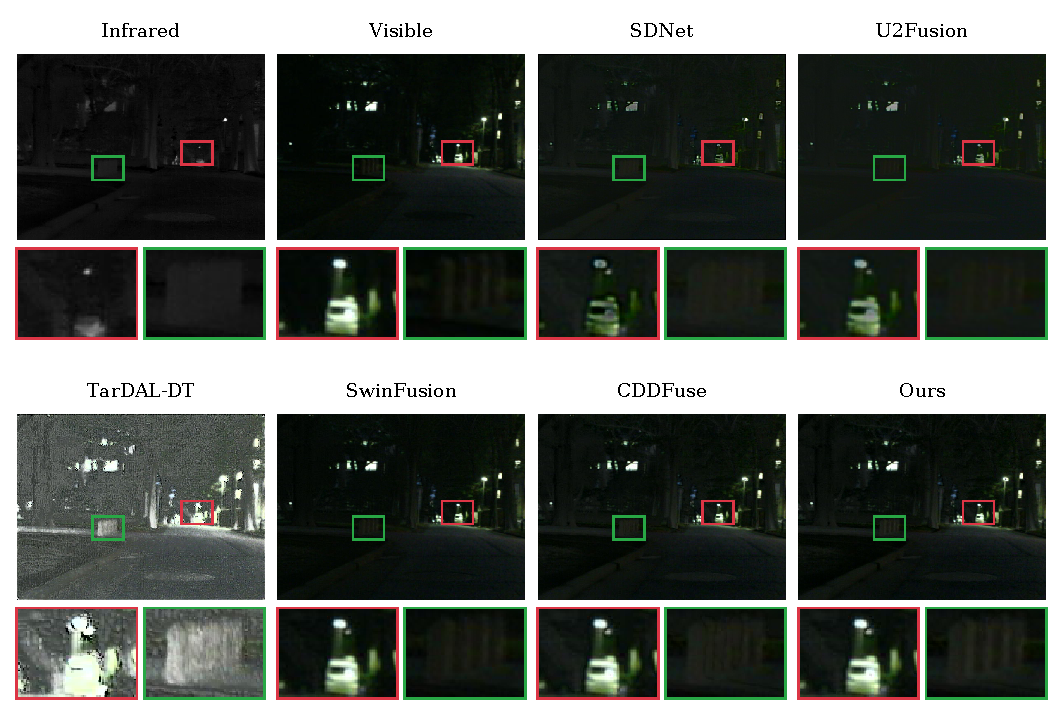
\includegraphics[width=0.98\textwidth]{figs/visual_sota_msrs.pdf}
\caption{Nighttime visual comparison. The red boxes enlarge a foreground target; the green boxes show background structures. Each full image is paired with the same two crops.}
\label{fig:visual_msrs}
\end{figure*}

\textbf{Daytime driving scene.}
\Cref{fig:visual_roadscene} contains a vehicle with different infrared and visible appearances, together with a bright building facade. SwinFusion's result has low contrast in the highlighted facade, making window and traffic-signal details less distinct. SCMFuse combines a visible rear-window boundary with thermal cues around the vehicle and retains the traffic signal and window outlines in the green crop. CDDFuse provides a similarly detailed result; the dataset-level VIF and $Q^{AB/F}$ improvements offer broader evidence for the proposed method than either selected image alone.

\begin{figure*}[!t]
\centering
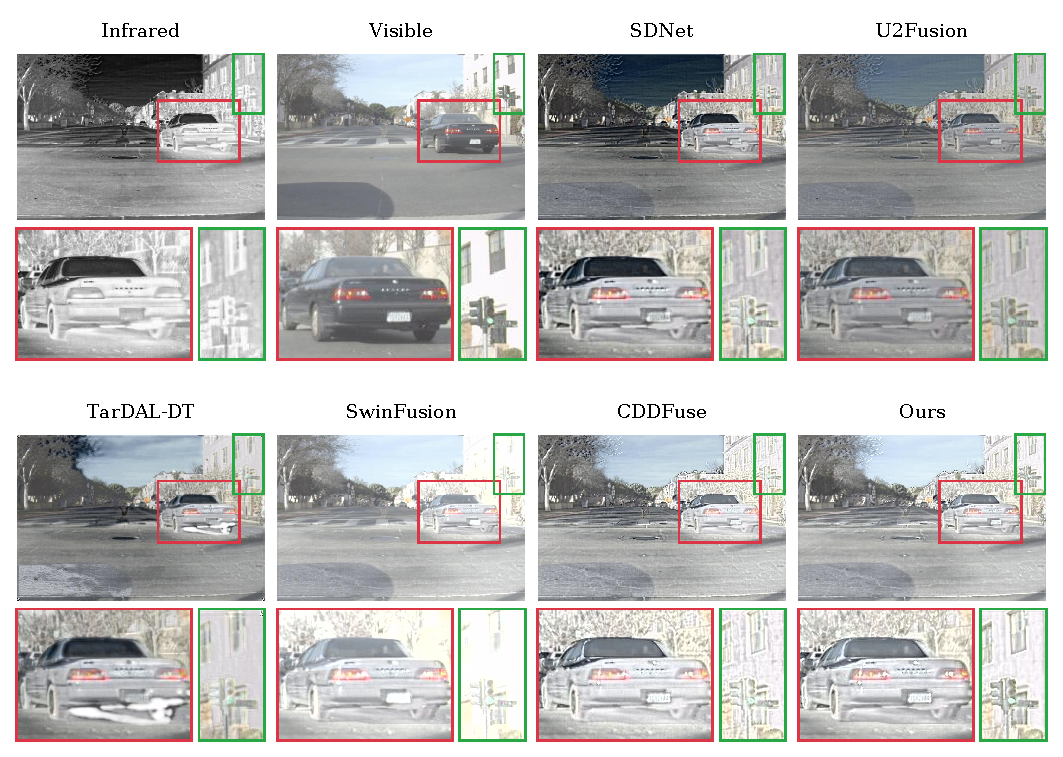
\includegraphics[width=0.98\textwidth]{figs/visual_sota_roadscene.pdf}
\caption{Daytime visual comparison. The red boxes highlight the vehicle, and the green boxes cover the traffic signal and building windows. Enlarged regions use the same locations across methods.}
\label{fig:visual_roadscene}
\end{figure*}
% Visual assets are retained without altering any fused result. Exact Ours checkpoint and TarDAL-DT/TarDAL mapping are recorded as provenance items in the final editorial review.

\subsection{Computational Efficiency}\label{subsec:efficiency}
\begin{table}[!t]
\centering
\caption{Reported model size and computational cost. Ours-P and Ours-C share the inference graph.}
\label{tab:complexity}
\small
\setlength{\tabcolsep}{8pt}
\begin{tabular}{@{}lrr@{}}
\toprule
Method & Params (M) & FLOPs (G)\\
\midrule
DenseFuse & 0.074 & 11.532\\
FusionGAN & 0.926 & 124.775\\
DIDFuse & 0.261 & 48.620\\
SDNet & 0.029 & 3.746\\
U2Fusion & 0.659 & 86.341\\
TarDAL & 0.297 & 38.768\\
SeAFusion & 0.167 & 21.758\\
SwinFusion & 0.974 & 149.365\\
FusionMamba & 164.539 & 92.076\\
CDDFuse & 1.188 & 235.716\\
Ours-P / Ours-C & 0.473 & 87.837\\
\bottomrule
\end{tabular}
\end{table}

\begin{table}[!t]
\centering
\caption{Training efficiency on the RTX 5070 Ti: 40 Phase I epochs and 80 Phase II epochs. Total time and speedup are rounded from the measured epoch durations.}
\label{tab:training}
\small
\setlength{\tabcolsep}{4pt}
\begin{tabular}{@{}lrrrr@{}}
\toprule
 & \multicolumn{2}{c}{Time (s/epoch)} & Total & Speedup\\
\cmidrule(lr){2-3}
Model & Phase I & Phase II & (h) & ($\times$)\\
\midrule
Baseline & 230.5 & 216.0 & 7.36 & 1.00\\
L (+SGC) & \textbf{126.4} & \textbf{111.7} & \textbf{3.89} & \textbf{1.89}\\
Ours-P & 138.1 & 135.6 & 4.55 & 1.62\\
Ours-C & 142.0 & 141.2 & 4.72 & 1.56\\
\bottomrule
\end{tabular}
\end{table}

\textbf{Model size and operations.}
As shown in \cref{tab:complexity}, SCMFuse uses $0.473$ M parameters and $87.837$ G FLOPs under the reported profile, compared with $1.188$ M and $235.716$ G for CDDFuse. The reductions are $60.2\%$ and $62.7\%$, respectively. Ours-P and Ours-C have identical model complexity because the additional supervision is evaluated only during training. Although several convolutional methods are smaller, SCMFuse combines its compact model with stronger fusion scores across multiple fidelity and structure metrics.
% Profiling input dimensions, operator coverage, and the specific baseline implementations were not independently remeasured; see final review.

The SGC and SCM Blocks contain point-wise projections with $\mathcal O(HWD^2)$ cost when kernel sizes, expansion ratios, state dimensions, and head counts are fixed. Both scale linearly with spatial size for fixed $D$. Pooling confines the four-directional scan to one-quarter of the original token count per direction for even image dimensions, while the main residual path remains full resolution. The resulting runtime benefit is evaluated through the measured latency rather than inferred from asymptotic complexity alone.

\textbf{Training and inference.}
\Cref{tab:training} shows that the lightweight configuration L reduces total training time from $7.36$ to $3.89$ hours. Ours-P and Ours-C require approximately $4.55$ and $4.72$ hours, corresponding to $1.62\times$ and $1.56\times$ acceleration. The contrast--structure terms add a small training overhead to the same inference architecture.

\begin{table*}[!t]
\centering
\caption{Inference latency (ms) and throughput (FPS) on the RTX 5070 Ti. Mean speedup is the arithmetic mean of the three dataset-specific latency ratios relative to CDDFuse. Best entries are bold.}
\label{tab:efficiency_comparison}
\small
\setlength{\tabcolsep}{9pt}
\begin{tabular}{@{}lrrrrrrr@{}}
\toprule
 & \multicolumn{2}{c}{MSRS} & \multicolumn{2}{c}{TNO} & \multicolumn{2}{c}{RoadScene} & Mean\\
\cmidrule(lr){2-3}\cmidrule(lr){4-5}\cmidrule(lr){6-7}
Model & ms & FPS & ms & FPS & ms & FPS & speedup\\
\midrule
SwinFusion & 412.5 & 2.42 & 1240.0 & 0.81 & 1385.2 & 0.72 & $0.80\times$\\
CDDFuse & 309.1 & 3.24 & 1017.3 & 0.98 & 1153.8 & 0.87 & $1.00\times$\\
L (+SGC) & \textbf{142.6} & \textbf{7.01} & 333.6 & 3.00 & 542.7 & 1.84 & $2.45\times$\\
Ours-P & 161.0 & 6.21 & \textbf{304.9} & \textbf{3.28} & \textbf{373.1} & \textbf{2.68} & $\mathbf{2.78\times}$\\
Ours-C & 160.6 & 6.23 & 310.4 & 3.22 & 373.9 & 2.67 & $2.76\times$\\
\bottomrule
\end{tabular}
\end{table*}

\Cref{tab:efficiency_comparison} reports inference time across the three datasets. Ours-C reduces MSRS latency from $309.1$ to $160.6$ ms, TNO latency from $1017.3$ to $310.4$ ms, and RoadScene latency from $1153.8$ to $373.9$ ms. Averaging these dataset-specific latency ratios gives a $2.76\times$ mean speedup. Ours-P achieves $2.78\times$. The two configurations share the same inference design; their small timing difference does not establish a runtime benefit from changing the loss. The efficiency gain is most pronounced on TNO and RoadScene, where the baseline has the largest latency.
% Timing precision, input resolutions, CUDA synchronization, I/O exclusion, warm-up and repetitions require the original benchmark script for full reproducibility.

\subsection{Ablation Studies}\label{subsec:ablation_study}
\textbf{Progressive configurations.}
\Cref{tab:main_ablation} evaluates four configurations: \textbf{B}, the CDDFuse baseline; \textbf{L}, B with the SGC-based encoder and hybrid decoder; \textbf{A}, L with the SCM Block, DGF, and MGF; and \textbf{F}, A with the proposed supervision. A and F correspond to Ours-P and Ours-C. Each step tests a defined set of changes within the complete framework.
% Historical mapping: B=Exp-0; L=Exp-1; A=manuscript Exp-2 / historical Exp-3_v2; F=manuscript Exp-3 / loss-enabled Exp-3_v2.
\begin{table*}[!t]
\centering
\caption{Progressive ablation. B: CDDFuse; L: lightweight encoder--decoder; A: L with the SCM Block, DGF, and MGF; F: A with the proposed supervision. A and F correspond to Ours-P and Ours-C. The best and second-best values are marked in \best{bold red} and \second{underlined blue}. Ties follow the displayed precision; all metrics are higher-is-better.}
\label{tab:main_ablation}
\small
\setlength{\tabcolsep}{7pt}
\begin{tabular}{@{}lrrrrrrrr@{}}
\toprule
Method & EN & SD & SF & MI & SCD & VIF & $Q^{AB/F}$ & SSIM\\
\midrule
\multicolumn{9}{c}{\textbf{MSRS}}\\
\midrule
B (Baseline) & 6.69 & 42.99 & \second{11.71} & \best{3.68} & 1.61 & \best{1.06} & \second{0.72} & \second{0.99}\\
L (+SGC) & \second{6.70} & \second{43.16} & 11.67 & \second{3.62} & \second{1.65} & \best{1.06} & \second{0.72} & \best{1.00}\\
A (+SCM and gates) & \second{6.70} & 43.02 & \best{11.75} & 3.35 & 1.61 & \best{1.06} & \best{0.73} & 0.98\\
F (+Supervision) & \best{6.73} & \best{43.31} & 11.66 & 3.45 & \best{1.70} & \best{1.06} & \best{0.73} & \second{0.99}\\
\midrule
\multicolumn{9}{c}{\textbf{TNO}}\\
\midrule
B (Baseline) & \second{7.10} & \second{45.47} & \second{13.49} & 2.41 & 1.64 & 0.79 & 0.56 & \second{0.98}\\
L (+SGC) & \best{7.11} & \best{45.73} & \best{13.50} & 2.35 & \best{1.72} & 0.81 & 0.56 & \best{1.01}\\
A (+SCM and gates) & 7.08 & 43.46 & 13.14 & \best{2.72} & 1.60 & \best{0.87} & \best{0.61} & 0.97\\
F (+Supervision) & 7.08 & 43.63 & 13.26 & \second{2.48} & \second{1.71} & \second{0.83} & \second{0.60} & \best{1.01}\\
\midrule
\multicolumn{9}{c}{\textbf{RoadScene}}\\
\midrule
B (Baseline) & 7.30 & 48.78 & \best{15.88} & 2.47 & 1.68 & 0.69 & 0.56 & \second{0.95}\\
L (+SGC) & \best{7.37} & \best{51.35} & 15.73 & 2.39 & \best{1.76} & 0.70 & 0.55 & \best{0.96}\\
A (+SCM and gates) & 7.30 & 49.17 & 15.71 & \best{2.62} & 1.62 & \best{0.77} & \best{0.62} & 0.92\\
F (+Supervision) & \second{7.32} & \second{50.12} & \second{15.84} & \second{2.54} & \second{1.72} & \second{0.75} & \second{0.61} & \second{0.95}\\
\bottomrule
\end{tabular}
\end{table*}


\textbf{Local processing (B $\to$ L).}
Replacing the shallow processing and decoder configuration increases throughput from $3.24$ to $7.01$ FPS on MSRS, $0.98$ to $3.00$ FPS on TNO, and $0.87$ to $1.84$ FPS on RoadScene. SD and SCD also increase on all three datasets, while VIF and $Q^{AB/F}$ remain close to the baseline. This establishes an efficient starting point for the deeper architectural changes.

\textbf{Space--channel modeling and fusion (L $\to$ A).}
The combined addition of the SCM Block and learned fusion gates improves TNO MI from $2.35$ to $2.72$, VIF from $0.81$ to $0.87$, and $Q^{AB/F}$ from $0.56$ to $0.61$. The corresponding RoadScene values increase from $2.39$, $0.70$, and $0.55$ to $2.62$, $0.77$, and $0.62$. MSRS $Q^{AB/F}$ rises to $0.73$. These results support the joint spatial--channel and aggregation design, particularly for transfer to the two other datasets.

\textbf{Proposed supervision (A $\to$ F).}
Adding the new objective raises SCD from $1.61/1.60/1.62$ to $1.70/1.71/1.72$ on MSRS/TNO/RoadScene. SD increases from $43.02/43.46/49.17$ to $43.31/43.63/50.12$, and SSIM from $0.98/0.97/0.92$ to $0.99/1.01/0.95$. MSRS MI also improves from $3.35$ to $3.45$. The full objective retains the MSRS VIF and $Q^{AB/F}$ values and trades a small portion of the TNO/RoadScene perceptual scores for higher structural correlation and contrast. The comparison evaluates the supervision package as a whole, rather than the contribution of each individual loss term.

\textbf{Intermediate architectural designs.}
\Cref{tab:mamba_variants} compares two exploratory designs with the final original-loss architecture. Variant V1 downsamples the base trunk and uses a scan-output channel normalization while retaining MDTA at the reduced resolution. Variant V2 uses channel scaling, removes MDTA, and applies an additional feature-rescaling operation. The final design retains the full-resolution residual stream and MDTA, and omits that feature rescaling.
\begin{table}[!t]
\centering
\caption{Intermediate base/fusion designs trained with the original objective. V1/V2 denote exploratory variants; Final is Ours-P. Best values are in bold.}
\label{tab:mamba_variants}
\small
\setlength{\tabcolsep}{4pt}
\begin{tabular}{@{}llrrrr@{}}
\toprule
Dataset & Variant & SD & MI & VIF & $Q^{AB/F}$\\
\midrule
MSRS & V1 & \textbf{43.15} & \textbf{3.45} & \textbf{1.06} & 0.72\\
 & V2 & 42.90 & 3.28 & \textbf{1.06} & \textbf{0.73}\\
 & Final & 43.02 & 3.35 & \textbf{1.06} & \textbf{0.73}\\
\midrule
TNO & V1 & \textbf{44.71} & 2.38 & 0.81 & 0.56\\
 & V2 & 44.22 & 2.53 & 0.83 & \textbf{0.61}\\
 & Final & 43.46 & \textbf{2.72} & \textbf{0.87} & \textbf{0.61}\\
\midrule
RoadScene & V1 & 48.51 & 2.50 & 0.72 & 0.58\\
 & V2 & \textbf{49.47} & 2.44 & 0.75 & 0.61\\
 & Final & 49.17 & \textbf{2.62} & \textbf{0.77} & \textbf{0.62}\\
\bottomrule
\end{tabular}
\end{table}

The final design achieves the highest TNO and RoadScene MI and VIF among these alternatives, with $Q^{AB/F}$ also leading or tying. Because several choices differ jointly, this comparison supports the integrated design rather than isolating normalization, resolution, or attention effects. Together with the progressive study, these results support the choice of the final architecture.

\FloatBarrier
\section{Conclusion}\label{sec:conclusion}
We presented SCMFuse, an efficient infrared and visible image fusion framework based on dual-branch feature decomposition. SGC Blocks reduce the cost of shallow encoding and reconstruction, and the SCM Block combines spatial state-space scanning with full-resolution residual features and channel attention. DGF and MGF adapt the aggregation of base and detail representations. The training objective adds intra-modal decorrelation, local structural correlation, and global--local contrast retention to the intensity and gradient supervision.

Experiments on MSRS, TNO, and RoadScene show improved structural correlation and competitive fusion quality with $60.2\%$ fewer parameters and $62.7\%$ fewer FLOPs than CDDFuse. The full model provides $1.56\times$ training acceleration and $2.76\times$ mean inference speedup, with particularly clear gains in TNO and RoadScene edge-related fidelity. The two training configurations provide different balances between structural correlation, contrast, and information fidelity. Future work will examine robustness to imperfect registration and the effect of the fused images on downstream perception.


% ==================== 参考文献 ====================
{\small
\bibliographystyle{IEEEtran}
\bibliography{refs}
}

\end{document}
